\documentclass[11pt,a4paper]{article}

\usepackage[utf8]{inputenc}
\usepackage[T1]{fontenc}
\usepackage{amsmath}
\usepackage{amssymb}
\usepackage{amsthm}
\usepackage{doi}
\usepackage{hyperref}
\usepackage[margin=2.5cm]{geometry}
\usepackage{booktabs}
\usepackage{graphicx}
\usepackage{enumitem}

\theoremstyle{plain}
\newtheorem{theorem}{Theorem}[section]
\newtheorem{lemma}[theorem]{Lemma}
\newtheorem{corollary}[theorem]{Corollary}
\newtheorem{proposition}[theorem]{Proposition}
\theoremstyle{definition}
\newtheorem{definition}[theorem]{Definition}
\newtheorem{hypothesis}[theorem]{Hypothesis}
\theoremstyle{remark}
\newtheorem{remark}[theorem]{Remark}

\newcommand{\Omegaspace}{\Omega}
\newcommand{\Obs}{\mathcal{O}}

\title{Projective Information Loss and Fibre Erasure\\
in Admissible Non-Injective Projection}
\author{J\'er\^ome Beau\\[4pt]
\small Independent Researcher, Puteaux, France\\
\small \texttt{jerome.beau@cosmochrony.org}}
\date{2026}

\begin{document}

  \maketitle

  \begin{abstract}
    We establish a fibre-erasure theorem for the admissible coarse-graining hierarchy
    of the Cosmochrony spectral programme~\cite{Beau2026l,Beau2026m}.
    The non-injective projection $\Pi : \Omegaspace \to \Obs$ defines a residual
    fibre-information functional $I(c;\sigma(\ell))$,
    where $c$ is a Weil-block fibre label and $\sigma_c(\ell)$ is the BFS capacity
    profile at coarse-graining depth~$\ell$.
    Conditional on the structural sufficiency hypothesis~\textup{[H-suff]} ---
    that $\sigma(\ell)$ is a sufficient statistic for the hierarchy beyond~$\ell$,
    a condition numerically supported for $q \in \{61, 151, 211\}$
    (Section~\ref{sec:hsuff-test}) --- the data-processing inequality~\cite{CoverThomas2006}
    implies that $I(c;\sigma(\ell))$ is non-increasing in~$\ell$:
    fibre information is erased, not created, under admissible coarse-graining.
    This result is \emph{not} a $c$-theorem; it does not count effective degrees of freedom.
    It is a quantitative realisation of the ENI no-go theorem~\cite{Beau2026l}:
    non-injectivity of~$\Pi$ forces projective information loss,
    and the data-processing inequality makes this loss monotone and measurable.
    The inter-sector variance $\mathrm{Var}_c(\sigma_c(\ell))$ serves as a computable proxy;
    its restriction to $\mathrm{SU}(3)$ colour-triplets connects directly
    to hypothesis~[H-color]~\cite{Beau2026a35,Beau2026a36}.
  \end{abstract}

% TODO: add CoverThomas2006 to cosmochrony-bibliography.bib
% Cover, T.M., Thomas, J.A.: Elements of Information Theory, 2nd ed. Wiley (2006).

  \smallskip
  \noindent\textbf{Keywords.}
  non-injective projection;
  fibre erasure;
  admissible coarse-graining;
  data-processing inequality;
  information monotone;
  BFS capacity;
  spectral admissibility;
  projective information loss;
  Weil representation;
  Heisenberg group;
  [H-color]

  \newpage
  \tableofcontents

  \newpage

  \section{Introduction}
    \label{sec:intro}

    The ENI no-go theorem~\cite{Beau2026l} establishes a fundamental structural fact:
    genuine emergence is necessarily non-injective.
    Any surjective map $\Pi : \Omegaspace \to \Obs$ satisfying the projective-emergent
    conditions carries a strictly positive projection entropy~$S_\Pi > 0$:
    information about the microscopic representative is irrecoverably lost at the effective level.
    This is a qualitative result.
    It identifies the structure of information loss but says nothing about how this loss
    is distributed across a hierarchy of resolutions.

    The Cosmochrony spectral programme~\cite{Beau2026a1,Beau2026a2} provides a concrete
    realisation of this hierarchy.
    For each prime~$q$, the BFS capacity profiles~$\sigma_c(\ell)$, indexed by
    Weil-block fibre label~$c$ and coarse-graining depth~$\ell$,
    track the residual projective capacity of block~$c$ as the BFS cascade advances.
    Numerical campaigns across $q \in \{61, 151, 211, 307\}$ reveal a consistent pattern:
    inter-sector variance collapses as depth increases, and the profiles converge
    toward a universal profile~$\sigma^*$ approached in the limit $q \to \infty$
    (Section~\ref{sec:axis-disambig}).
    Hypothesis~[H-color]~\cite{Beau2026a35,Beau2026a36} identifies one specific instance
    of this convergence: the $\mathrm{SU}(3)$ colour-triplet sectors
    $\{c, \omega c, \omega^2 c\}$ become indistinguishable at the effective level
    for $q \equiv 1 \pmod{3}$.

    This paper addresses the following question:
    can the qualitative ENI no-go and the quantitative spectral convergence be connected
    by a principled information-theoretic structure?
    We show that the answer is yes, conditional on the structural sufficiency
    hypothesis~\textup{[H-suff]}:
    the residual fibre-information functional $I(c;\sigma(\ell))$
    is non-increasing in the coarse-graining depth~$\ell$,
    by the data-processing inequality~\cite{CoverThomas2006}.
    The result is conditional, not unconditional:
    \textup{[H-suff]} is strongly motivated (Remark~\ref{rem:suff-not-adhoc}),
    numerically supported for $q \in \{61, 151, 211\}$ (Section~\ref{sec:hsuff-test}),
    but not yet proved analytically.

    Two structural distinctions are essential before proceeding.
    First, the coarse-graining axis~$\ell$ is distinct from and orthogonal to
    the temporal cascade axis~$n$ of the PTO paper~\cite{Beau2026pto}:
    see Table~\ref{tab:axes} and Remark~\ref{rem:axes}.
    Second, as stated in Section~\ref{sec:claims}, ENI alone does not imply monotonicity;
    the hierarchical structure of~\textup{[H-suff]} and~\textup{[H-sg]} is
    the informational content this paper contributes beyond ENI.

    \subsection{Contributions and non-claims}
      \label{sec:claims}

      This paper establishes, conditional on hypotheses~\textup{[H-suff]}
      and~\textup{[H-sg]} (Section~\ref{sec:semigroup}):
      \begin{enumerate}[label=(\roman*)]
\item a monotone information functional $I(c;\sigma(\ell))$
for the BFS coarse-graining hierarchy (Theorem~\ref{thm:erasure});
\item its non-increase under depth-increment, via the data-processing inequality;
\item the identification of $I(c;\sigma(\ell)) = 0$
as the fibre-erasure equilibrium condition (Corollary~\ref{cor:fixedpoint}).
      \end{enumerate}
      This paper does \emph{not} establish:
      \begin{enumerate}[label=(\roman*)]
\item a $c$-theorem or analogue (no counting of effective degrees of freedom;
see open problem~\textup{[O-2]});
\item hypothesis~\textup{[H-suff]} itself
(stated and motivated; numerically supported for $q \in \{61, 151, 211\}$;
analytical proof remains open, see~\textup{[O-1]});
\item the semigroup hypothesis~\textup{[H-sg]}
(stated and motivated; see open problem~\textup{[O-1]}).
      \end{enumerate}

      \paragraph{Strict disclaimer.}
        This result should not be called a $c$-theorem.
        It is a \emph{fibre-erasure theorem}:
        the monotone measures the loss of residual fibre-label information under
        admissible coarse-graining.
        A $c$-theorem-type statement would require an additional counting principle
        for effective degrees of freedom, which is not established here and is listed
        as open problem~\textup{[O-2]} in Section~\ref{sec:open}.

      \paragraph{ENI versus monotonicity.}
        ENI~\cite{Beau2026l} establishes that information is structurally lost under
        non-injective projection, but does not by itself imply any monotone hierarchy
        over the coarse-graining scale~$\ell$.
        The monotonicity of Theorem~\ref{thm:erasure} requires the additional
        hierarchical structure encoded in~\textup{[H-suff]} and~\textup{[H-sg]}:
        these are the informational content this paper contributes beyond ENI.

  \subsection{Programme placement}
    \label{sec:placement}

    The present paper occupies a hub position in the programme.
    ENI~\cite{Beau2026l} and Foundation~\cite{Beau2026m} provide the foundational input:
    the non-injective projection~$\Pi$, the Weil-fibre realisation,
    and the projection entropy~$S_\Pi$.
    The spectral admissibility programme~\cite{Beau2026a1,Beau2026a2} provides the
    operational hierarchy: the BFS capacity profiles~$\sigma_c(\ell)$ and their
    numerical campaigns, including the O31--O32
    investigation~\cite{Beau2026a35,Beau2026a36}.
    This paper connects these two branches by translating the ENI projection
    entropy into the operational functional~$I(c;\sigma(\ell))$
    and identifying spectral convergence~$\sigma_c \to \sigma^*$
    as the thermodynamic universal profile (Section~\ref{sec:axis-disambig}).
    The PTO paper~\cite{Beau2026pto} handles the complementary temporal axis~$n$
    (Table~\ref{tab:axes});
    the two papers are structurally orthogonal and together constitute
    the information-theoretic architecture of the admissibility cascade.

  \section{Framework}
  \label{sec:framework}

  \subsection{Non-injective projection and fibre structure}
    \label{sec:fibre}

    We recall the setting of~\cite{Beau2026l,Beau2026m}.

    \begin{definition}[Non-injective projection and fibre]
      \label{def:projection}
      A \emph{projective description} is a surjective map $\Pi : \Omegaspace \to \Obs$
      such that $\Obs$ carries no microstate-resolving structure independent of~$\Pi$.
      The \emph{fibre} over $o \in \Obs$ is
      $\Pi^{-1}(o) = \{\,\omega \in \Omegaspace : \Pi(\omega) = o\,\}$.
      The \emph{projection entropy} is
      $S_\Pi = \mathbb{E}_{o}[\,\log|\Pi^{-1}(o)|\,] \geq 0$,
      with $S_\Pi > 0$ whenever $\Pi$ is non-injective
      \textup{(ENI Theorem~2.1,~\cite{Beau2026l})}.
    \end{definition}

    In the spectral realisation~\cite{Beau2026m}, the fibre structure is implemented
    via the Weil representation $V_\rho$ of
    $\mathrm{Heis}_3(\mathbb{Z}/q\mathbb{Z})$ for a prime~$q$.
    The minimal non-injectivity is the parity involution $c \leftrightarrow q - c$:
    Weil blocks $\rho_c$ and $\rho_{q-c}$ map to the same effective observable class.
    The \emph{fibre label} $c \in \{1,\ldots,(q-1)/2\}$
    indexes blocks within an equivalence class under~$\Pi$.

  \subsection{The BFS coarse-graining hierarchy}
    \label{sec:bfs}

    \begin{definition}[BFS capacity profile]
      \label{def:bfs}
      For a prime~$q$, a fibre label~$c$, and BFS depth $\ell \in \mathbb{N}$,
      the \emph{BFS capacity profile} $\sigma_c(\ell) \in [0,1]$ is the normalised
      residual projective capacity of block~$c$ at depth~$\ell$ along the
      Heisenberg Cayley graph BFS cascade~\cite{Beau2026a1,Beau2026a2}.
      The \emph{pair observable} is
      $\sigma_{\mathrm{pair}}(\ell) = \sigma_c(\ell)\cdot\sigma_{q-c}(\ell)$
      on conjugate pair $(c,q-c)$.
    \end{definition}

    For a prime~$q$, the Heisenberg group $\mathrm{Heis}_3(\mathbb{Z}/q\mathbb{Z})$
    carries a Cayley graph whose BFS shells~$B_\ell$ grow as $|B_\ell| \sim \ell^4$
    in the Heisenberg regime~\cite{Beau2026a1}.
    The capacity profile~$\sigma_c(\ell)$ measures the residual Gram-Schmidt span
    of Weil block~$\rho_c$ not yet exhausted at shell depth~$\ell$:
    it starts at $\sigma_c(0) = 1$ and decreases toward~$0$
    as BFS saturation is approached.
    The depth parameter~$\ell \in \mathbb{N}$ is discrete;
    the coarse-graining semigroup of Section~\ref{sec:semigroup}
    therefore acts on a discrete monoid, not a continuous scale.

  \subsection{Three-axis separation}
    \label{sec:axes}

    \begin{table}[h]
      \centering
      \begin{tabular}{lll}
        \toprule
        Axis & Parameter & Role \\
        \midrule
        Coarse-graining / resolution
        & $\ell$ (BFS depth/window)
        & coarse-graining hierarchy; carries $I(c;\sigma(\ell))$; this paper \\
        Thermodynamic / continuum
        & $q \to \infty$
        & Limit for $\sigma^*$; established numerically (Section~\ref{sec:axis-disambig}) \\
        Temporal / cascade
        & $n$ (cascade step)
        & Projective time; carries $I(n)$ of~\cite{Beau2026pto} \\
        \bottomrule
      \end{tabular}
      \caption{The three distinct axes of the observable hierarchy.
      The coarse-graining axis~$\ell$ is the support of this paper.
      The temporal axis~$n$ is the support of PTO~\cite{Beau2026pto}.
      The continuum axis $q \to \infty$ is the thermodynamic limit in which
      the fixed point~$\sigma^*$ is approached;
      Section~\ref{sec:axis-disambig} establishes this numerically.}
      \label{tab:axes}
    \end{table}

    \begin{remark}[Cascade and coarse-graining are orthogonal]
      \label{rem:axes}
      The admissible cascade $U_0 \to U_1 \to \cdots$ defines the temporal axis~$n$
      and is \emph{not} an RG flow.
      RG-like behaviour is carried by~$\Pi$ and the semigroup $\{G_{\ell' \leftarrow \ell}\}$
      on the $\ell$-axis.
      The cascade \emph{enlarges} the admissible space as temporal ordering advances;
      an RG flow toward the IR \emph{reduces} effective degrees of freedom.
      These are distinct phenomena on orthogonal axes.
      The fibre-erasure fixed point~$\sigma^*$ lives on the thermodynamic axis:
      it is approached as $q \to \infty$ with $\mathrm{O}(q^{-1/2})$ corrections,
      not as a Wilsonian $\ell$-limit at fixed~$q$
      (Section~\ref{sec:axis-disambig}).
    \end{remark}

  \subsection{The coarse-graining semigroup}
    \label{sec:semigroup}

    \begin{definition}[Coarse-graining channel]
      \label{def:channel}
      For $\ell' > \ell$, the \emph{coarse-graining channel}
      $G_{\ell' \leftarrow \ell} : \sigma(\ell) \mapsto \sigma(\ell')$
      is the map sending the BFS capacity profile at depth~$\ell$ to the profile
      at depth~$\ell'$.
    \end{definition}

    \begin{hypothesis}[\textup{[H-sg]}: semigroup property]
      \label{hyp:sg}
      The coarse-graining channels satisfy
      \begin{equation}
        \label{eq:sg}
        G_{\ell_3 \leftarrow \ell_2} \circ G_{\ell_2 \leftarrow \ell_1}
        = G_{\ell_3 \leftarrow \ell_1}
        \qquad \text{for all } \ell_1 < \ell_2 < \ell_3.
      \end{equation}
    \end{hypothesis}

    Hypothesis~\textup{[H-sg]} is plausible from the nested structure of BFS shells:
    the subgraph induced by~$B_{\ell_1}$ is contained in that induced by~$B_{\ell_2}$
    for $\ell_1 < \ell_2$,
    so the transition $\sigma(\ell_1) \to \sigma(\ell_2)$ can in principle be factored
    through~$\sigma(\ell_1)$ alone.
    Without~\textup{[H-sg]}, the data-processing inequality applied step-by-step
    via~\textup{[H-suff]} yields $I(c;\sigma(\ell+1)) \leq I(c;\sigma(\ell))$
    for each consecutive pair,
    but not the uniform statement of Theorem~\ref{thm:erasure} for all $\ell' > \ell$.
    Note that the semigroup acts on the space of observable descriptions,
    not on the static substrate~$\Omegaspace$:
    composability is a property of the coarse-graining of effective observables.

  \subsection{Probability measure on fibre labels}
    \label{sec:measure}

    \begin{definition}[Fibre-label measure]
      \label{def:measure}
      Let $\mu$ be a probability measure on $\{c : 1 \le c \le (q-1)/2\}$.
      Two canonical choices are used:
      \begin{enumerate}[label=(\roman*)]
\item \emph{Uniform}: $\mu(c) = 2/(q-1)$ for all~$c$.
\item \emph{Triplet-uniform} (for $q \equiv 1 \pmod{3}$):
$\mu$ uniform on $\{c,\,\omega c,\,\omega^2 c\}$,
where $\omega$ is a primitive cube root of unity modulo~$q$;
used in the [H-color] context~\cite{Beau2026a35,Beau2026a36}.
      \end{enumerate}
    \end{definition}

    The choice of~$\mu$ does not affect the monotonicity of $I(c;\sigma(\ell))$
    (which holds for any fixed measure by DPI),
    but affects its value and the interpretation of the fixed point.

  \section{Structural Sufficiency and the Markov Property}
  \label{sec:suff}

  \begin{hypothesis}[\textup{[H-suff]}: structural sufficiency]
    \label{hyp:suff}
    For all $\ell' > \ell$, the coarse-graining channel $G_{\ell' \leftarrow \ell}$
    is conditionally independent of the fibre label~$c$ given $\sigma(\ell)$:
    \begin{equation}
      \label{eq:markov}
      c \;\longrightarrow\; \sigma(\ell) \;\longrightarrow\; \sigma(\ell').
    \end{equation}
    That is, $\sigma(\ell)$ is a \emph{sufficient statistic} for~$\sigma(\ell')$
    with respect to the fibre label~$c$.
    The term ``sufficient'' is used in the information-theoretic sense:
    all information in~$\sigma(\ell)$ that is predictive of~$\sigma(\ell')$
    is already fully encoded; no additional knowledge of~$c$ reduces
    the uncertainty in~$\sigma(\ell')$ beyond what $\sigma(\ell)$ already captures.
  \end{hypothesis}

  \begin{remark}[Interpretive status of~\textup{[H-suff]}]
    \label{rem:suff-not-adhoc}
    Hypothesis~\textup{[H-suff]} is not introduced solely to enable the DPI.
    It is the informational reformulation of an effective closure property already
    implicit throughout the spectral admissibility programme:
    if~\textup{[H-suff]} failed --- if BFS dynamics at depth~$\ell'$ re-accessed
    label information not encoded in~$\sigma(\ell)$ ---
    then $\sigma_c(\ell)$ would not constitute stable effective observables under~$\Pi$,
    and the convergence $\sigma_c \to \sigma^*$, the plateau structure
    across $q \in \{61, 151, 211, 307\}$,
    and the [H-color] campaign~\cite{Beau2026a35,Beau2026a36}
    would be structurally very difficult to account for.
    More precisely,~\textup{[H-suff]} is the condition that the BFS observable~$\sigma(\ell)$
    constitutes a \emph{complete summary} of the fibre structure at resolution~$\ell$:
    the projection~$\Pi$ has already collapsed the relevant fibre information
    at each level of the hierarchy, and no deeper BFS step retrieves it.
    This is exactly what the non-injectivity of~$\Pi$ (ENI~\cite{Beau2026l}) demands
    at the effective level: fibre information is not gradually re-injected
    as coarse-graining proceeds, but is collapsed once and for all by~$\Pi$.
    In this sense,~\textup{[H-suff]} makes explicit, in information-theoretic language,
    a structural commitment already implicit in the programme's use
    of~$\sigma_c(\ell)$ as an effective observable.
  \end{remark}

  \begin{remark}[Status of~\textup{[H-suff]}]
    \label{rem:suff-status}
    Hypothesis~\textup{[H-suff]} is strongly motivated by Remark~\ref{rem:suff-not-adhoc}
    and is compatible with all known spectral results.
    A permutation-based Spearman test on BFS capacity data for $q \in \{61, 151, 211\}$
    yields no significant $c$-dependence in step-by-step residuals at any tested depth
    (Section~\ref{sec:hsuff-test}), providing numerical evidence for~\textup{[H-suff]}.
    Analytical proof remains open; see open problem~\textup{[O-1]}.
  \end{remark}

  \begin{remark}[Why~\textup{[H-suff]} is load-bearing]
    \label{rem:loadsuff}
    If hypothesis~\textup{[H-suff]} fails for some pair $(\ell,\ell')$ ---
    that is, if $\sigma(\ell')$ depends on~$c$ beyond its dependence on~$\sigma(\ell)$
    --- then no structural information monotone of the form
    $I(c;\sigma(\ell')) \leq I(c;\sigma(\ell))$ can be guaranteed.
    If $p(\sigma(\ell') \mid \sigma(\ell), c) \neq p(\sigma(\ell') \mid \sigma(\ell))$
    for some~$c$, then the chain $c \to \sigma(\ell) \to \sigma(\ell')$ is not Markov,
    and the data-processing inequality does not apply.
    This is not a limitation of the proof technique;
    it reflects the genuine logical dependence of the monotonicity on the Markov structure.
  \end{remark}

  A proof of~\textup{[H-suff]} would establish that the BFS depth-increment
  kernel $p(\sigma(\ell+1) \mid \sigma(\ell), c)$ is independent of the fibre label~$c$.
  Structurally, this would follow from the fact that the BFS recursion on the
  Heisenberg Cayley graph is governed by the group geometry ---
  shared across all fibre labels up to conjugation ---
  and the Born-Infeld admissibility constraint,
  rather than by the specific character of block~$c$.
  A partial result is already in hand:
  the conjugation symmetry $\rho_c \cong \rho_{q-c}$ ensures
  $\sigma_c(\ell) = \sigma_{q-c}(\ell)$ within each conjugate pair,
  consistent with~\textup{[H-suff]} at the pair level.
  The full extension requires showing that cross-pair dynamics also factors
  through~$\sigma(\ell)$.

  The full extent of~\textup{[H-suff]} --- including cross-pair dynamics ---
  has been tested numerically for $q \in \{61, 151, 211\}$;
  see Section~\ref{sec:hsuff-test}.

  \section{The Fibre-Erasure Theorem}
  \label{sec:erasure}

  \subsection{The information functional}

    \begin{definition}[Residual fibre information]
      \label{def:info}
      The \emph{residual fibre information} at depth~$\ell$ is
      \begin{equation}
        \label{eq:mutual}
        I(c;\sigma(\ell))
        = H(c) - H(c \mid \sigma(\ell))
        = H(\sigma(\ell)) - H(\sigma(\ell) \mid c),
      \end{equation}
      where $H(\cdot)$ denotes Shannon entropy with respect to measure~$\mu$.
    \end{definition}

    \begin{remark}[Physical interpretation]
      \label{rem:info-interp}
      $I(c;\sigma(\ell)) = 0$ if and only if $\sigma(\ell) \perp c$:
      the BFS profile carries no information about the microscopic fibre representative.
      This is the operational statement of fibre erasure under~$\Pi$.
    \end{remark}

  \subsection{Main theorem}

    \begin{theorem}[Fibre-Erasure Theorem]
      \label{thm:erasure}
      Assume hypotheses~\textup{[H-suff]} (Hypothesis~\ref{hyp:suff})
      and~\textup{[H-sg]} (Hypothesis~\ref{hyp:sg}).
      Then for all $\ell' > \ell \geq 0$:
      \begin{equation}
        \label{eq:erasure}
        I\bigl(c;\sigma(\ell')\bigr) \;\leq\; I\bigl(c;\sigma(\ell)\bigr).
      \end{equation}
      In particular, $I(c;\sigma(\ell))$ is non-increasing in~$\ell$
      and converges to a limit $I_\infty \geq 0$.
    \end{theorem}

    \begin{proof}[Proof sketch]
By~\textup{[H-suff]}, the triple $(c,\sigma(\ell),\sigma(\ell'))$ forms
a Markov chain~\eqref{eq:markov}.
The data-processing inequality~\cite{CoverThomas2006}
applied to this chain gives~\eqref{eq:erasure} directly.
Composability~\textup{[H-sg]} extends the inequality from $\ell' = \ell + 1$
to all $\ell' > \ell$.
    \end{proof}

    \begin{corollary}[Fibre-erasure equilibrium condition]
      \label{cor:fixedpoint}
      Under the hypotheses of Theorem~\ref{thm:erasure},
      $I(c;\sigma(\ell)) = 0$ if and only if $\sigma(\ell) \perp c$.
      This is the \emph{fibre-erasure equilibrium}: the coarse-graining
      has fully collapsed the fibre-label information.
      It is realised by the thermodynamic universal profile~$\sigma^*$
      in the limit $q \to \infty$ (Remark~\ref{rem:fixedpoint-thermo}).
    \end{corollary}

    \paragraph{Explicit disclaimer.}
      Theorem~\ref{thm:erasure} is \emph{not} a $c$-theorem.
      At the fibre-erasure equilibrium, $I_\infty = 0$ does not count any
      effective degrees of freedom.
      A $c$-theorem analog requires a separate counting functional;
      see open problem~\textup{[O-2]}.

  \subsection{Information decomposition and programme connections}
  \label{sec:decomp}

  By the chain rule for entropy:
  \begin{equation}
    \label{eq:decomp}
    H\bigl(\sigma(\ell)\bigr)
    = H\bigl(\sigma(\ell) \mid c\bigr) + I\bigl(c;\sigma(\ell)\bigr).
  \end{equation}
  Here $I(c;\sigma(\ell))$ is the fibre-erasure functional (Theorem~\ref{thm:erasure}),
  monotone non-increasing in~$\ell$;
  $H(\sigma(\ell) \mid c)$ is the intrinsic entropy of the observable conditioned on
  the fibre label, and is the natural candidate for a counting monotone~\textup{[O-2]}.

  \begin{remark}[Connection to PTO and axis orthogonality]
    \label{rem:pto}
    The temporal monotone $I(n) = \sigma_{\mathrm{pair}}(0) - \sigma_{\mathrm{pair}}(n)$
    of~\cite{Beau2026pto} lives on the temporal axis~$n$ (Table~\ref{tab:axes}).
    The present $I(c;\sigma(\ell))$ lives on the coarse-graining axis~$\ell$.
    They measure distinct phenomena on orthogonal axes and should not be conflated.
  \end{remark}

  \section{Numerical Proxies and Spectral Programme Connections}
  \label{sec:numerics}

  \subsection{Inter-sector variance as proxy}

    \begin{definition}[Inter-sector variance]
      \label{def:variance}
      The \emph{inter-sector variance} at depth~$\ell$ is
      \begin{equation}
        \label{eq:variance}
        \mathcal{V}(\ell)
        = \mathrm{Var}_c\bigl(\sigma_c(\ell)\bigr)
        = \mathbb{E}_c\bigl[\sigma_c(\ell)^2\bigr]
        - \bigl(\mathbb{E}_c[\sigma_c(\ell)]\bigr)^2.
      \end{equation}
    \end{definition}

    $\mathcal{V}(\ell) = 0$ is a necessary condition for $I(c;\sigma(\ell)) = 0$,
    but $\mathcal{V}$ is \emph{not} guaranteed to be monotone in~$\ell$.
    Non-monotone behaviour of~$\mathcal{V}$ would not contradict Theorem~\ref{thm:erasure};
    it would indicate that variance is an imperfect surrogate for~$I(c;\sigma(\ell))$.

  \subsection{Triplet variance and \textup{[H-color]}}

    For $q \equiv 1 \pmod{3}$, the \emph{triplet-restricted variance} is
    \begin{equation}
      \label{eq:tripvar}
      \mathcal{V}_{\mathrm{triplet}}(\ell)
      = \mathrm{Var}\bigl(\sigma_c(\ell),\;
      \sigma_{\omega c}(\ell),\; \sigma_{\omega^2 c}(\ell)\bigr),
    \end{equation}
    averaged over colour triplets.

    \begin{remark}[\textup{[H-color]} as a fibre-erasure statement]
      \label{rem:hcolor}
      Hypothesis~[H-color] of~\cite{Beau2026a35,Beau2026a36} asserts
      $\sigma_c(\ell) = \sigma_{\omega c}(\ell) = \sigma_{\omega^2 c}(\ell)$
      for $q \equiv 1 \pmod{3}$,
      which is precisely $\mathcal{V}_{\mathrm{triplet}}(\ell) = 0$ and,
      under~\textup{[H-suff]}, $I_{\mathrm{triplet}}(c;\sigma(\ell)) = 0$.
      The fibre-erasure theorem provides the information-theoretic framework within
      which [H-color] is a special case:
      the colour label becomes unobservable at the effective level.
      The triplet-restricted variance is already computable from the
      $q \in \{61, 151, 211, 307\}$ runs of O32~\cite{Beau2026a36}.
    \end{remark}

  \subsection{Numerical evidence for~\textup{[H-suff]}}
    \label{sec:hsuff-test}

    Hypothesis~\textup{[H-suff]} was tested numerically on the BFS capacity data
    from the O25 pipeline~\cite{Beau2026a1,Beau2026a2}
    for $q \in \{61, 151, 211\}$.
    For each depth step $\ell \to \ell+1$,
    the $k$-nearest-neighbour regression residuals
    $e_c = \sigma_c(\ell+1) - \hat{f}(\sigma_c(\ell))$
    are computed from all $q-1$ block-averaged mean trajectories,
    where $\hat{f}$ is estimated without reference to~$c$.
    The Spearman correlation $|\rho(e_c, c)|$ is then computed
    and compared to a permutation null (500 shuffles of~$c$),
    yielding a right-tail $p$-value and a standardised $z$-score.
    Under~\textup{[H-suff]}, the residuals~$e_c$ should be independent
    of~$c$, and $|\rho|$ should be statistically indistinguishable
    from zero at every depth.

    \begin{table}[h]
      \centering
      \begin{tabular}{lrrrr}
        \toprule
        $q$ & depths tested & $|\rho|_{\max}$ & $z$-score max
        & signif.\ ($p < 0.05$) \\
        \midrule
        61  & 10 & 0.169 & 0.78 & 0/10 \\
        151 & 37 & 0.123 & 1.05 & 0/37 \\
        211 & 49 & 0.120 & 1.55 & 0/49 \\
        \bottomrule
      \end{tabular}
      \caption{Spearman test of conditional independence
        $\sigma(\ell+1) \perp c \mid \sigma(\ell)$ on BFS capacity data
        for $q \in \{61, 151, 211\}$.
        $|\rho|_{\max}$: maximum absolute Spearman correlation
        between residuals and the fibre label over all tested depth steps.
        $z$-score: standardised deviation from the permutation null.
        Significant: number of depth steps with $p < 0.05$; zero in all cases.}
      \label{tab:hsuff}
    \end{table}

    For all three primes and across all depth steps tested,
    $|\rho(e_c, c)|$ does not exceed $0.17$
    and no depth step yields $p < 0.05$.
    The results, shown in Figure~\ref{fig:hsuff}, are consistent
    with the permutation null throughout:
    no systematic $c$-dependence in the step-by-step residuals is detected.

    \begin{figure}[h]
      \centering
      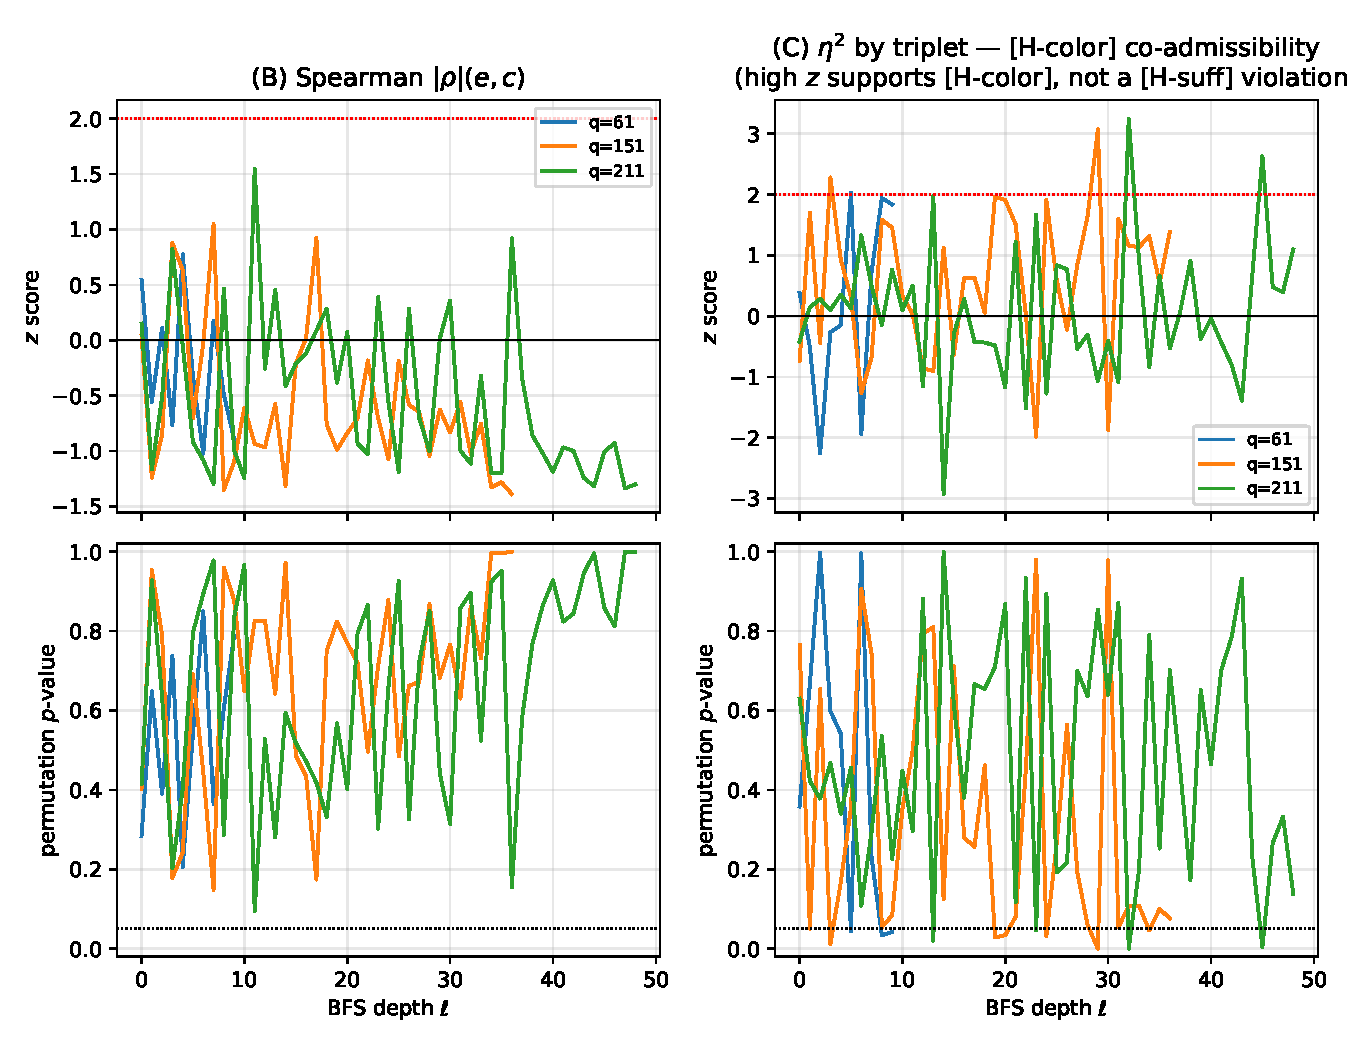
\includegraphics[width=\textwidth]{hsuff_vs_depth}
      \caption{Numerical test of~\textup{[H-suff]} for $q \in \{61, 151, 211\}$.
      \textbf{Left panels~(B):} Spearman $|\rho|(e_c, c)$ test
        ($z$-scores and $p$-values vs BFS depth~$\ell$).
        All $z$-scores lie below the $z = 2$ threshold (dashed red);
        no depth is significant.
        \textbf{Right panels~(C):} leave-triplet-out $\eta^2$ test
        grouped by $\mathrm{SU}(3)$ colour triplet for $q \equiv 1 \pmod{3}$;
        this measures [H-color] co-admissibility quality and does not test
        \textup{[H-suff]} directly (see text).}
      \label{fig:hsuff}
    \end{figure}

    These results constitute numerical evidence that the BFS depth-increment dynamics
    does not depend on the fibre label~$c$ beyond the capacity profile~$\sigma(\ell)$,
    consistent with~\textup{[H-suff]}.

    \paragraph{Limitations.}
      The test is limited by the available data:
      the O25 pipeline~\cite{Beau2026a1,Beau2026a2} stores only the mean BFS capacity
      profile averaged over $M$~block samples per fibre label;
      per-block trajectories would enable a more powerful categorical test.
      No full O25 run is currently available for $q = 307$,
      though [H-color] at $q = 307$ has been confirmed directly
      by O32~\cite{Beau2026a36}.

    \paragraph{[H-color] co-admissibility diagnostic.}
      The leave-triplet-out $\eta^2$ test (panel~C of Figure~\ref{fig:hsuff})
      detects strong within-triplet residual correlation at $q = 151$
      ($z_{\max} = 3.07$) and moderately at $q = 211$ ($z_{\max} = 3.25$),
      consistent with the [H-color] co-admissibility established
      by O32~\cite{Beau2026a36}: triplet members share equal $\sigma$ profiles,
      giving equal residuals after leave-triplet-out regression.
      This is not evidence against~\textup{[H-suff]}; it is an incidental
      corroboration of [H-color].
      The signal increases with better [H-color] quality:
      $q = 151$ has the smallest inter-triplet variance ratio
      ($R_{\mathrm{var}} = 0.71 \times 10^{-3}$) of the tested primes,
      consistent with the strongest triplet signal.

      \clearpage
  \subsection{Axis disambiguation: the fixed point is thermodynamic}
  \label{sec:axis-disambig}

  The question of whether the fibre-erasure fixed point~$\sigma^*$ ---
  the configuration where $I(c;\sigma(\ell)) = 0$ and fibre-label information
  is fully collapsed --- is approached as a limit in the coarse-graining
  depth~$\ell$ at fixed~$q$ (a Wilsonian fixed point of the semigroup
  $\{G_{\ell' \leftarrow \ell}\}$) or only in the thermodynamic limit $q \to \infty$
  was investigated numerically on the BFS capacity data for $q \in \{61, 151, 211\}$.
  Two complementary diagnostics were computed.

  \paragraph{Coefficient of variation.}
    The scale-free inter-sector spread
    \begin{equation}
      \label{eq:cv}
      \mathrm{CV}(\ell)
      = \frac{\mathrm{std}_c\bigl(\sigma_c(\ell)\bigr)}
      {\mathrm{mean}_c\bigl(\sigma_c(\ell)\bigr)}
    \end{equation}
    equals $\mathrm{std}(A_c)/\mathrm{mean}(A_c)$, a depth-independent constant,
    if and only if profiles differ purely by amplitude:
    $\sigma_c(\ell) = A_c\,\sigma^*(\ell)$.
    Decrease of~$\mathrm{CV}(\ell)$ to zero would indicate convergence to a common
    profile, i.e.\ a Wilsonian fixed point at fixed~$q$.
    The data show~$\mathrm{CV}(\ell)$ starting small at the fitting-window entry
    ($0.045$--$0.079$ across $q \in \{61, 151, 211\}$)
    and growing throughout the pre-saturation regime at all three primes
    (Figure~\ref{fig:o4}, left panels);
    no plateau or decrease toward zero is observed.
    This rules out Wilsonian convergence at fixed~$q$.

  \paragraph{Amplitude-ratio test.}
    For 20 random pairs $(c, c')$, the coefficient of variation of the ratio
    $\sigma_c(\ell)/\sigma_{c'}(\ell)$ over depth measures shape differences
    beyond amplitude scaling.
    Table~\ref{tab:o4} shows this quantity decreasing with~$q$.
    \begin{table}[h]
      \centering
      \begin{tabular}{lrr}
        \toprule
        $q$ & ratio-CV mean & ratio-CV std \\
        \midrule
        61  & 0.156 & 0.069 \\
        151 & 0.065 & 0.021 \\
        211 & 0.062 & 0.025 \\
        \bottomrule
      \end{tabular}
      \caption{Amplitude-ratio CV over 20 random pairs $(c, c')$:
      coefficient of variation of $\sigma_c(\ell)/\sigma_{c'}(\ell)$
        over depth in the pre-saturation regime.
        The decrease with~$q$ is consistent with $\mathrm{O}(q^{-1/2})$
        shape corrections from U1 universality~\cite{Beau2026a1,Beau2026a2}.}
      \label{tab:o4}
    \end{table}
    The trend from $q = 61$ ($0.156$) to $q \in \{151, 211\}$ ($0.065$--$0.062$)
    is consistent with $\mathrm{O}(q^{-1/2})$ corrections
    from U1 universality~\cite{Beau2026a1,Beau2026a2}:
    at larger~$q$, profiles approach a common shape.

  \paragraph{Cross-$q$ mean profile comparison.}
    After normalising each mean profile by its value at the fitting-window
    start~$\ell_0 = n_0$,
    the profiles for $q = 151$ and $q = 211$ are nearly identical,
    while $q = 61$ decays more rapidly (Figure~\ref{fig:o4}, right panel).
    No collapse onto a single $q$-universal curve is observed at finite~$q$.

    \begin{figure}[h]
      \centering
      \begin{minipage}[t]{0.56\textwidth}
        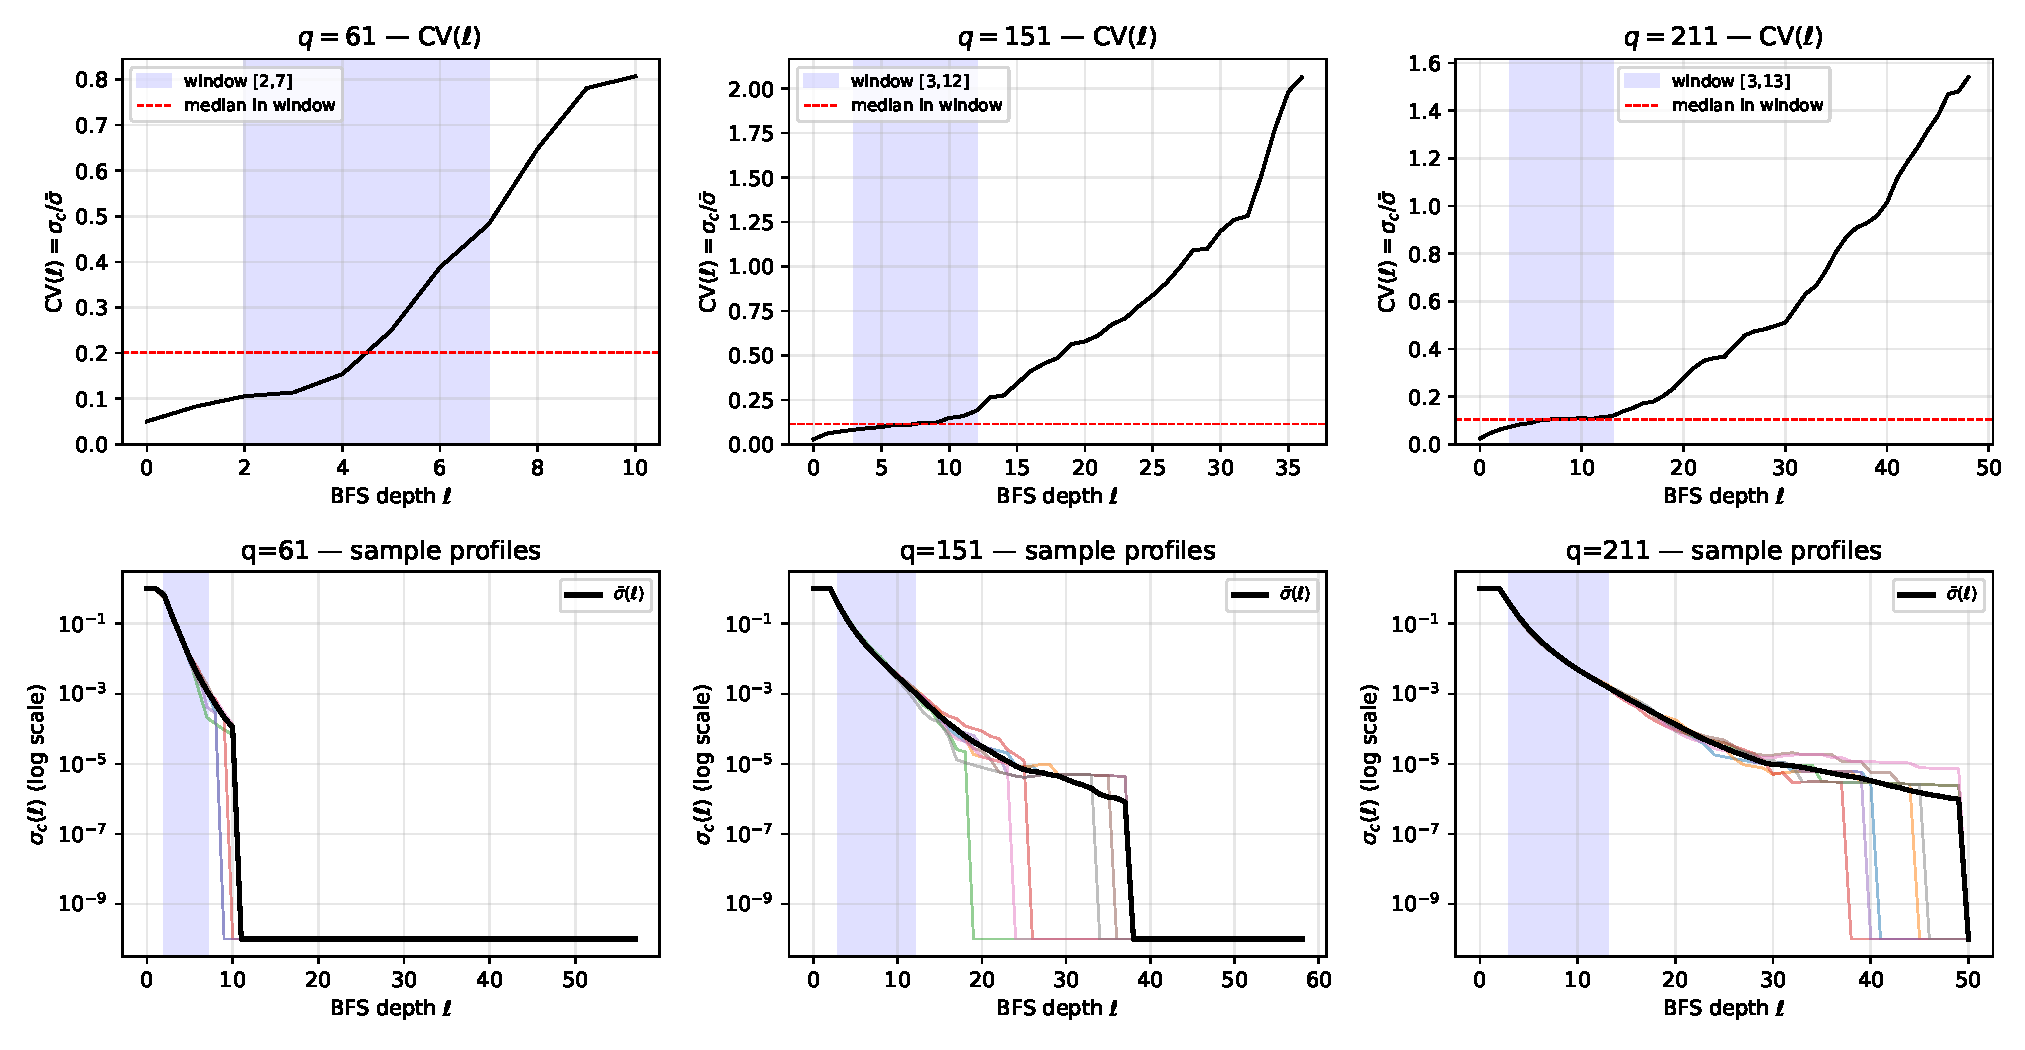
\includegraphics[width=\textwidth]{o4_cv_profiles}
      \end{minipage}%
      \hfill
      \begin{minipage}[t]{0.41\textwidth}
        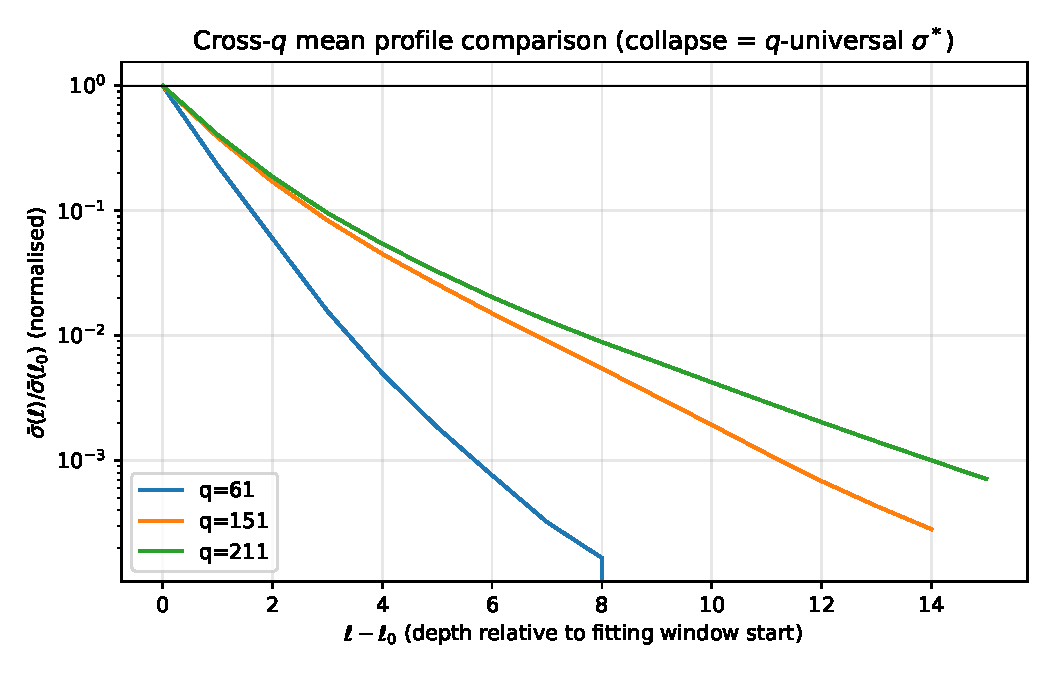
\includegraphics[width=\textwidth]{o4_cross_q}
      \end{minipage}
      \caption{\textbf{Left:} $\mathrm{CV}(\ell)$ (top row) and sample profiles
      on a log scale (bottom row) for $q \in \{61,151,211\}$.
      Blue band: fitting window~$[n_0, n_1]$.
        $\mathrm{CV}(\ell)$ grows monotonically throughout the pre-saturation regime;
        the sharp rise beyond the window is a saturation artefact
        (different $c$ values reach $\sigma_c \to 0$ at different depths).
        No plateau or decrease toward zero is observed.
        \textbf{Right:} cross-$q$ mean profiles normalised at~$\ell_0 = n_0$.
        The $q = 151$ and $q = 211$ profiles are nearly identical;
        $q = 61$ decays faster.
        The absence of collapse confirms that $\sigma^*$ requires $q \to \infty$.}
      \label{fig:o4}
    \end{figure}

    These results establish that~$\sigma^*$ is a thermodynamic limit object:
    it is approached as $q \to \infty$ with $\mathrm{O}(q^{-1/2})$ amplitude corrections
    from U1 universality, not as a Wilsonian $\ell$-limit at fixed~$q$.
    At finite~$q$, approximate fixed points~$\sigma^*(q)$ exist with $c$-dependent
    amplitude corrections~$A_c$ that vanish as $q \to \infty$;
    the universal fixed point requires the continuum limit.

    \begin{remark}[Residual fibre information at finite~$q$; terminology]
      \label{rem:fixedpoint-thermo}
      Theorem~\ref{thm:erasure} and Corollary~\ref{cor:fixedpoint} hold for any fixed~$q$:
      their conclusion is that $I(c;\sigma(\ell))$ is non-increasing; they do not require
      the equilibrium condition to be reached.
      At finite~$q$, a residual $I(c;\sigma(\ell)) > 0$ persists at all depths,
      reflecting the $c$-dependent amplitude corrections~$A_c$.

      A terminological precision is warranted.
      The \emph{fibre-erasure fixed point} of Corollary~\ref{cor:fixedpoint}
      is the equilibrium condition $I(c;\sigma) = 0$ on the information functional ---
      not a fixed point of the semigroup $\{G_{\ell' \leftarrow \ell}\}$,
      which has no non-trivial fixed point at finite~$q$
      (all profiles eventually reach $\sigma_c(\ell) \to 0$ by BFS saturation).
      The universal profile~$\sigma^*$ realising this equilibrium condition is
      therefore better understood as the \emph{thermodynamic universal profile}:
      $\sigma^* = \lim_{q \to \infty} \sigma^*(q)$,
      where $\sigma^*(q)$ are approximate equilibria at finite~$q$
      with $I(c;\sigma^*(q)) > 0$,
      approaching exact equilibrium only in the projective continuum limit $q \to \infty$
      (Conjecture~4.7 of~\cite{Beau2026q5b}).
    \end{remark}

    \clearpage
  \section{Open Problems}
  \label{sec:open}

  \begin{description}[style=nextline]
\item[\textup{[O-1]} Analytical proof of~\textup{[H-suff]}.]
Establish that the BFS depth-increment map $G_{\ell+1 \leftarrow \ell}$
is a Markov kernel on~$\sigma$:
the transition $p(\sigma(\ell+1) \mid \sigma(\ell), c)$ is independent of~$c$.
Numerical evidence is available for $q \in \{61, 151, 211\}$
via the Spearman residual test of Section~\ref{sec:hsuff-test};
the analytical proof is the remaining open task.
The structural route would show that the BFS recursion depends on
the Heisenberg group geometry --- shared across all fibre labels
up to conjugation --- and the Born-Infeld admissibility constraint,
not on the specific character of block~$c$.

\item[\textup{[O-1b]} Proof of the semigroup hypothesis~\textup{[H-sg]}.]
Show that the coarse-graining channels compose as
$G_{\ell_3 \leftarrow \ell_2} \circ G_{\ell_2 \leftarrow \ell_1}
= G_{\ell_3 \leftarrow \ell_1}$ for all $\ell_1 < \ell_2 < \ell_3$.
Without~\textup{[H-sg]}, the data-processing inequality yields
step-by-step monotonicity (from each application of~\textup{[H-suff]})
but not the uniform statement of Theorem~\ref{thm:erasure}
for all $\ell' > \ell$.
Neither a numerical test nor an analytical proof is currently available.

\item[\textup{[O-2]} $c$-theorem analog via $H(\sigma(\ell))$.]
The decomposition~\eqref{eq:decomp} identifies
$H(\sigma(\ell) \mid c) = H(\sigma(\ell)) - I(c;\sigma(\ell))$
as a candidate counting monotone.
Establish its monotonicity in~$\ell$ and verify that its fixed-point value
counts effective degrees of freedom.
This would upgrade the fibre-erasure theorem to a genuine $c$-theorem analog.

\item[\textup{[O-3]} Temporal causal structure and emergent light cone.]
Define the temporal mutual information
$I_{\mathrm{temp}}(n,k) = I(U_n;\,U_{n+k})$
and the transfer entropy
$T(U_n \to U_{n+k}) = I(U_{n+k};\,U_n \mid U_{n-1},\ldots,U_0)$.
Their decay in~$k$ would yield an operational definition of the emergent forward
light cone on the temporal axis~$n$, orthogonal to the present paper.

  \end{description}

  \clearpage
  \bibliographystyle{plain}
  \bibliography{cosmochrony-bibliography,external-refs}

\end{document}
